\documentclass[12pt]{article}
\usepackage{url,graphicx,tabularx,array,geometry,enumitem,amsmath}
\setlength{\parskip}{1ex} %--skip lines between paragraphs
\setlength{\parindent}{0pt} %--don't indent paragraphs

%-- Commands for header
\renewcommand{\title}[1]{\textbf{#1}\\}
\renewcommand{\line}{\begin{tabularx}{\textwidth}{X>{\raggedleft}X}\hline\\\end{tabularx}\\[-0.5cm]}
\newcommand{\leftright}[2]{\begin{tabularx}{\textwidth}{X>{\raggedleft}X}#1%
& #2\\\end{tabularx}\\[-0.5cm]}

%\linespread{2} %-- Uncomment for Double Space
\begin{document}

\title{Digital Signal Processing - Assignment 4}
\line
\leftright{\today}{Stephanie Lund (2555914)\\Aljoscha Dietrich (2557976)} %-- left and right positions in the header

\section*{Exercise 1}

\subsection*{1.1}
The LPC technique predicts the next values from a given signal. It is based on the source-filter model of speech production, which states that speech is created by a source (the vocal cords) and an independent filter (the vocal tract) which creates resonances (formants). It is useful for encoding compressed speech.

\subsection*{1.2}
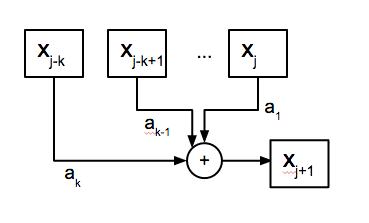
\includegraphics[scale=0.65]{hw4-2.png}
\begin{align*}
	x_{j+1} = \sum_{i=0}^{k} a_i x_{j-i}
\end{align*}

\subsection*{1.3}
The error equation for some measured $x_n$ is: $e_n = x_n + \sum_{i=1}^k a_i x_{n-i}$\\\\
We want to minimize the squared error $\mathcal{E} = E[ |e^2| ]$ with respect to the $a_k$ parameters.\\\\
Therefore, we want to minimize $\mathcal{E} = \frac{1}{N} \sum_{n=1}^N (x_n + \sum_{k=1}^p a_k x_{n-k})^2$\\\\

\subsection*{1.4}
We start with:
\begin{align*}
x(n) &= [-2, 0, 1, -1, 0, 2]\\
x(n+1) &= [0, 1, -1, 0, 2, 0]\\
x(n+2) &= [1, -1, 0, 2, 0, 0]\\
\end{align*}

Therefore, the autocorrelation matrix $R_{xx}$ with order 2 and window size of 6 is:
\begin{align*}
\begin{bmatrix}
r(0) & r(1) \\
r(1) & r(0)
\end{bmatrix}
= \begin{bmatrix}
10 & -1 \\
-1 & 10
\end{bmatrix}
\end{align*}

We want to solve for:

\begin{align*}
R_{xx}
\begin{bmatrix}
a_1 \\
a_2
\end{bmatrix}
=
-\begin{bmatrix}
r(1)\\
r(2)
\end{bmatrix}
=
\begin{bmatrix}
1 \\
4
\end{bmatrix}
\end{align*}

Solving this system, we get:

\begin{align*}
a_1 = \frac{14}{99} \qquad a_2 = \frac{41}{99}
\end{align*}

Therefore we have the prediction:
\begin{align*}
\hat{f[6]} = a_1 * f[5] + a_2 * f[4] = \frac{28}{99}
\end{align*}


\subsection*{1.5}
\begin{align*}
\hat{f[2]} = a_1 * f[1] + a_2 * f[0] =& -.83 \\
\hat{f[3]} =& .14\\
\hat{f[4]} =& .27\\
\hat{f[5]} =& -.41\\
\end{align*}

The errors are therefore:\\
\begin{align*}
e_2 = f[2] + \hat{f[2]} = 0&.17\\
e_3 = -0&.86\\
e_4 = 0&.27\\
e_5 = 1&.59
\end{align*}

\subsection*{1.6}
For order 4, we need to solve the equation:
\begin{align*}
\begin{bmatrix}
r(0) & r(1) & r(2) & r(3) & r(4) \\
r(1) & r(0) & r(1) & r(2) & r(3) \\
r(2) & r(1) & r(0) & r(1) & r(2)\\
r(3) & r(2) & r(1) & r(0) & r(1)\\
r{4} & r(3) & r(2) & r(1) & r(0)
\end{bmatrix}
\begin{bmatrix}
1\\
a_1\\
a_2\\
a_3\\
a_4
\end{bmatrix}
=
-\begin{bmatrix}
r(0)\\
r(1)\\
r(2)\\
r(3)\\
r(4)
\end{bmatrix}
\end{align*}

After solving for the r values, these are:
\begin{align*}
\begin{bmatrix}
10 & -1 & 4 & -4 & 0\\
-1 & 10 & -1 & 4 & -4\\
4 & -1 & 10 & -1 & 4 \\
-4 & 4 & -1 & 10 & -1\\
0 & -4 & 4 & -1 & 10
\end{bmatrix}
\begin{bmatrix}
1\\
a_1\\
a_2\\
a_3\\
a_4
\end{bmatrix}
=
\begin{bmatrix}
10\\
1\\
4\\
-4\\
0
\end{bmatrix}
\end{align*}

The Levinson-Durbin algorithm starts with solving the problem for order 1, then inductively solve for each following coefficient until we have reached our desired order (4 in this case).\\

The first step is then to solve:
\begin{align*}
\begin{bmatrix}
r(0) & r(1)\\
r(1) & r(0)
\end{bmatrix}
\begin{bmatrix}
1\\
a_1
\end{bmatrix}
=
\begin{bmatrix}
E_1\\
0
\end{bmatrix}
\end{align*}

We can solve this only using the second value, so that $r(1)*1 + r(0)*a_1 = 0$, therefore $a_1 = -\frac{r(1)}{r(0)} = \frac{1}{10}$.\\

From here, we can also solve for $E_1 = r(0) + r(1) * a_1 = 10 - \frac{1}{10} = 9.9$\\

The next step is to solve for $a_2$:


\end{document}